\documentclass[tikz,border=8pt]{standalone}
% Shared look for every TikZ diagram. Load with \input{../../tools/tikz-style.tex}
\usepackage[sfdefault]{roboto}
\usetikzlibrary{arrows.meta, positioning, shapes.geometric, calc, fit, backgrounds}
\definecolor{cblue}{HTML}{4C78A8}
\definecolor{corange}{HTML}{F58518}
\definecolor{cgreen}{HTML}{54A24B}
\definecolor{cred}{HTML}{E45756}
\definecolor{cpurple}{HTML}{B279A2}
\definecolor{cgrey}{HTML}{6B6B6B}
\tikzset{
  every picture/.style={font=\sffamily, line width=1.2pt},
  box/.style={draw=#1, fill=#1!12, rounded corners=4pt, align=center, inner sep=7pt, minimum height=1.1cm},
  box/.default=cgrey,
  arrow/.style={-{Stealth[length=3mm]}, draw=cgrey, line width=1.4pt},
  title/.style={font=\sffamily\bfseries\Large},
  note/.style={font=\sffamily\small, text=cgrey, align=center},
}
\AtBeginDocument{\hyphenpenalty=10000 \exhyphenpenalty=10000}

% MoveIt 2 (main): planners listed in one pipeline run in turn, each earlier result passed on as the reference
% trajectory (planning_pipeline.cpp); CHOMP takes it with fillTrajectory, STOMP with extractSeedTrajectory; the
% response adapter AddTimeOptimalParameterization times the path at the end.
\begin{document}
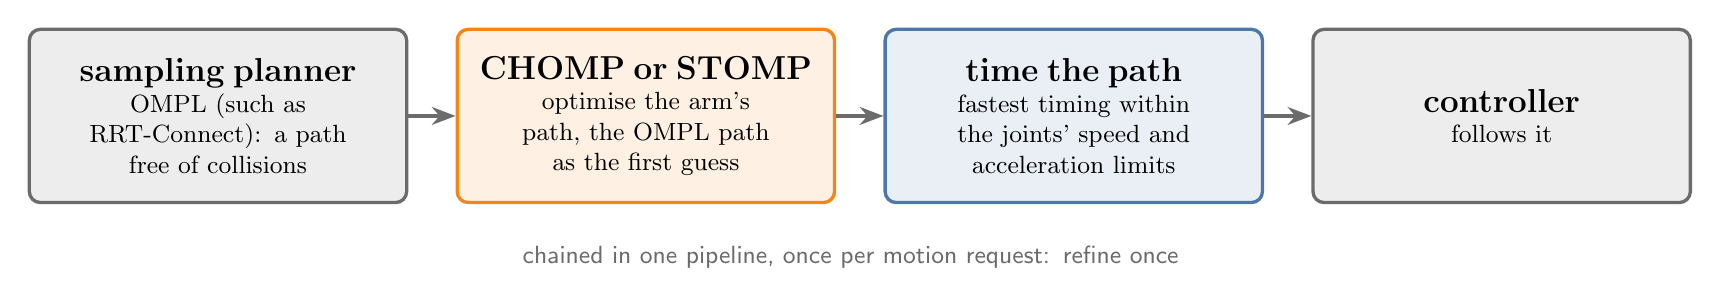
\begin{tikzpicture}[node distance=0.6cm,
  st/.style={box=#1, font=\small, minimum width=4.6cm, text width=4.3cm, minimum height=2.2cm}]
  \node[st=cgrey] (a) {{\large\textbf{sampling planner}}\\ OMPL (such as\\ RRT-Connect): a path\\ free of collisions};
  \node[st=corange, right=of a] (b) {{\large\textbf{CHOMP or STOMP}}\\ optimise the arm's\\ path, the OMPL path\\ as the first guess};
  \node[st=cblue, right=of b] (c) {{\large\textbf{time the path}}\\ fastest timing within\\ the joints' speed and\\ acceleration limits};
  \node[st=cgrey, right=of c] (d) {{\large\textbf{controller}}\\ follows it};
  \draw[arrow] (a) -- (b); \draw[arrow] (b) -- (c); \draw[arrow] (c) -- (d);
  \node[note, below=0.4cm of b, xshift=2.6cm, text width=10cm] {chained in one pipeline, once per motion request: refine once};
\end{tikzpicture}
\end{document}
